% Sections/1_introduction.tex
\section{Introduction}
Over 6.3 million vapes are discarded every week in the United Kingdom, despite the June 2025 national ban on single-use disposable vapes. \cite{defra_vape_ban_guidance_2025,letsrecycle_vapes_2025}. A vape, or e-cigarette, is an electronic nicotine delivery system that heats a liquid containing nicotine, flavourings, propylene glycol and other additives into an aerosol inhaled through a mouthpiece \cite{clevelandclinic_vaping_2022}. Once discarded, a vape becomes hazardous micro-litter because it contains a lithium-ion battery, metals, plastics, electronic components and e-liquid residues \cite{turner2024disposable_vapes_material,ngambo2023_ecig_environmental_impacts}. These components, if littered in nature, are hazardous because the battery can ignite if crushed or damaged while liquid residues can leach into the environment.

\begin{figure}[H]
    \centering
    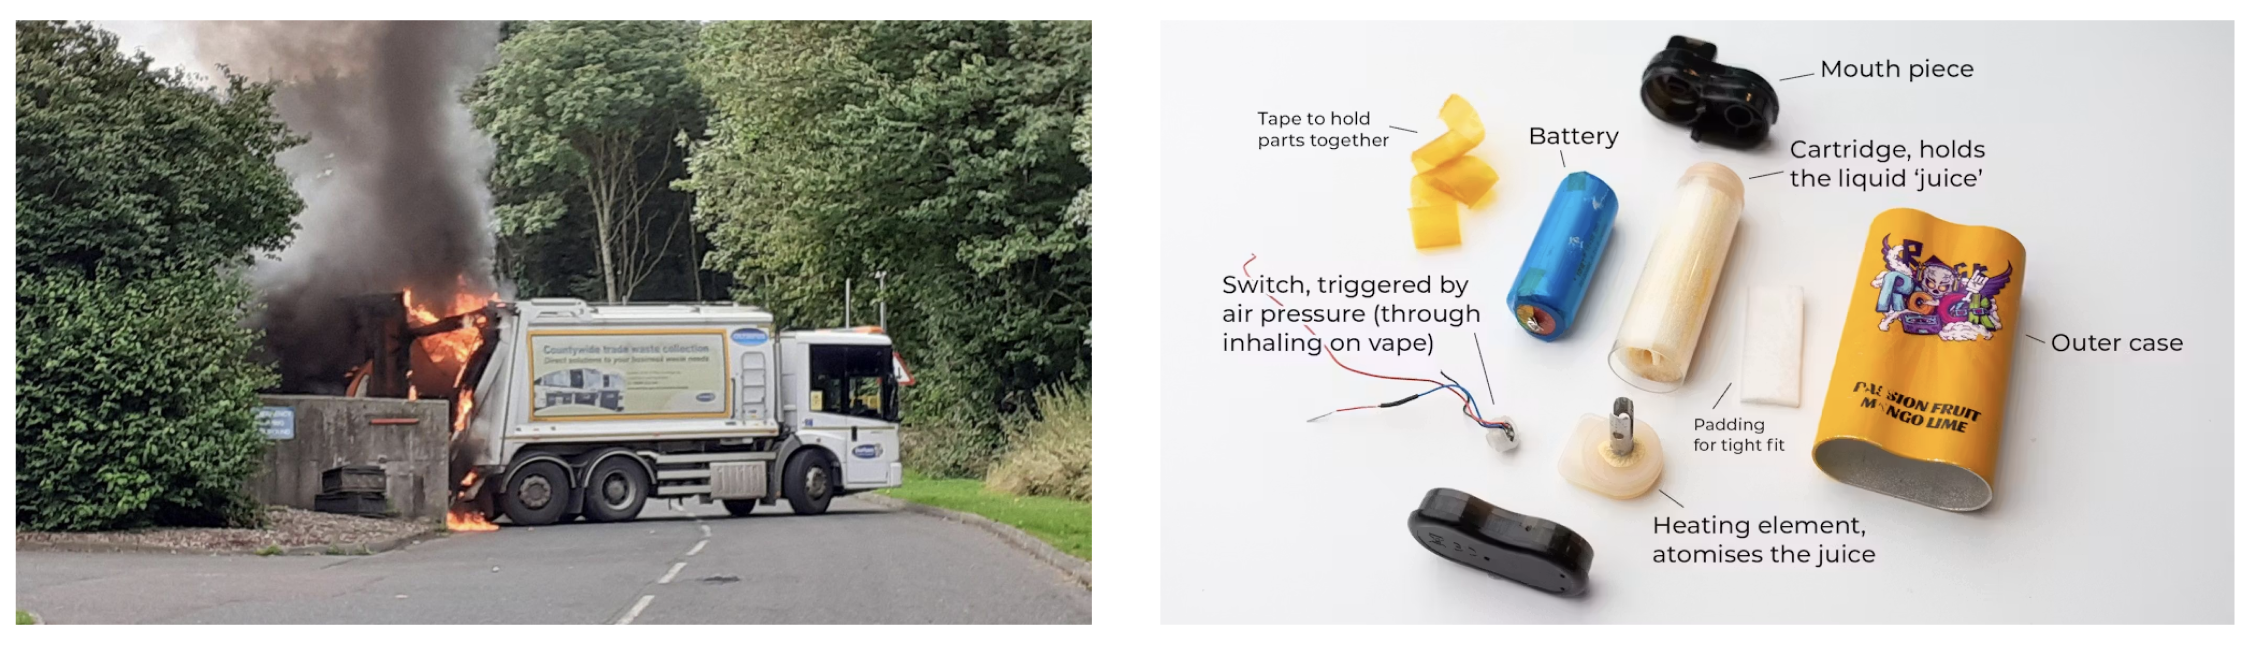
\includegraphics[width=0.7\linewidth]{vape fire.png}
    \caption{Left: fire caused by a disposable vape; right: vape exploded view.}
    \label{fig:intro_vape_fire_breakdown}
\end{figure}
The major institutional issue is not only frequent vape litter, but what happens after. Vapes are classified under the Waste Electrical and Electronic Equipment (WEEE) regime so should be separated from general waste and returned through appropriate recycling or take-back routes \cite{defra_vape_ban_guidance_2025}. However, this disposal pathway is not always understood. Material Focus reported that 47\% of vapers did not know that vapes could be recycled, increasing the likelihood that devices are littered, placed in public bins or mixed with ordinary waste \cite{letsrecycle_vapes_2025}. Once this happens, the embedded lithium-ion battery can be crushed or damaged during collection and processing. The National Fire Chiefs Council reported an epidemic level of 1,200 battery fires in UK bin lorries and waste sites in 2025-26, with vapes identified as a major waste-sector risk \cite{nfcc_battery_fires_2024}.

The practical challenge is that vapes do not visually signal the level of hazard they carry. Manual cleaning workflows depend on people visually scanning broad areas and deciding what to collect while moving through the environment. This works poorly for visually ambiguous micro-litter, particularly in public parks, towpaths and other open urban spaces where ground textures and vegetation can camouflage small objects. These spaces are also operationally relevant because they are routinely cleaned through visual inspection, are difficult to monitor continuously, and contain mixed ground textures that make small litter difficult to separate from the surrounding environment. If a vape is missed, the hazard remains in place or later enters an inappropriate waste stream.

Combining Unmanned Aerial Vehicles (UAVs) with computer vision offers a plausible way to improve this visibility stage. UAVs survey open space more efficiently than manual sweeps and can generate image evidence for downstream review. The UK Civil Aviation Authority's Drone Code allows small drones below 250g, or UK0-class drones, to operate closer to people and in residential, recreational, commercial and industrial areas, while still requiring safe operation and prohibiting flights over crowds \cite{caa_drone_code_where_fly_2026}. Prior UAV-litter research has also shown that aerial imagery and deep-learning detectors can identify rubbish in low-altitude images \cite{kraft2021uavvaste,bartolo2026litterreview}. 

However, existing UAV-litter work generally targets generic rubbish, bottles, marine debris or mixed small litter, rather than disposable vapes as a distinct hazardous micro-WEEE class. Further investigation showed that solving this problem requires more than training a detector. First, there is no mature, UAV-oriented vape litter dataset for UK urban environments. Second, the process of creating such a dataset is itself fragmented and inefficient: images must be sourced, reviewed, curated, annotated, described with environmental metadata, audited and exported before training can begin. Third, a model prediction is not operationally useful by itself. A vape detection must become an evidence-backed cleanup task if it is to support cleaners or waste organisations.

This dissertation frames a solution to these structural barriers through an interdisciplinary, systems-thinking approach. A Dataset Construction Engine (DCE) is created to provide the data infrastructure needed to construct a rich vape-litter dataset efficiently. A UAV vape litter dataset, UAVape, is then built and used to train a detector for vape-specific detection in UK urban environments. Finally, a vape cleanup planner is prototyped to explore how detections could be translated into cleaner-facing tasks.

This dissertation therefore revolves around the following research question:

\begin{quote}
    \textit{How can an integrated image-detection dataset construction engine, combined with deep-learning evaluation and workflow prototyping, overcome the structural barriers to identifying and operationalizing disposable vapes as hazardous micro-e-waste in UAV-oriented imagery for urban environments?}
\end{quote}

The core contributions are:

\begin{itemize}
    \item \textbf{The Dataset Construction Engine (DCE):} A novel image-detection data construction platform that centralizes image scraping, synthetic data creation, data upload, SAM2 semi-automated annotation, LLM-assisted metadata tagging, audit diagnostics and COCO/YOLO export. The DCE achieves faster annotation interaction times while preserving human review and dataset traceability.

    \item \textbf{The UAVape DCE Dataset:} A novel scraped non-litter vape dataset containing 2,905 vape-positive scraped images and 4,437 vape boxes, and a novel 2D synthetic vape-litter dataset containing 355 synthetic vape-positive composites and 355 vape boxes. Both were created through the DCE.

    \item \textbf{The UAVape Dataset:} A novel two-class vape/lighter UAV-oriented litter dataset containing 1,204 real UAV-oriented images, 1,328 vape boxes and 712 lighter boxes.

    \item \textbf{YOLO detector benchmark and data-source finding:} A unified model-selection benchmark across new-generation YOLO model families, model scales and input resolutions, followed by a controlled data-source ablation. The ablation showed that DCE-created scraped and synthetic data gave the strongest result when combined, while individual additions were mixed; the final selected recipe was then evaluated once on the sealed held-out test set.
    
    \item \textbf{The UAVape Vision Model:} A YOLO26s model trained using the selected UAVape data recipe, achieving a final held-out vape AP50 of 0.882 and vape AP50--95 of 0.685. The selected model used a two-class vape/lighter detector setup, with vape detection as the primary research target, and lighters as the auxiliary class.

    \item \textbf{Cleaner Workflow UI MVP:} A cleaner-facing workflow prototype that represents detections as evidence crops, confidence scores, map points, hazard labels and task statuses. Stakeholder walkthrough feedback indicated that such a phone-accessible workflow could improve vape-litter visibility and task clarity, while also revealing practical field constraints.
\end{itemize}

The dissertation is structured as follows: Section 2 reviews the UAV-litter literature, focusing on datasets, annotation, detection models, metrics and post-model operational gaps. Section 3 further investigates two deeper insights uncovered from the literature, motivating the DCE and Cleanup Planner. The design requirements then define the three workstreams. The following Method, Results and Discussion chapters report how each workstream was implemented, evaluated and interpreted.
